\chapter{监督微调与续训退化}\label{监督微调与续训退化}

\section{监督微调 SFT 用示范塑造助手行为}\label{监督微调 SFT 用示范塑造助手行为}

回到最初的方程题，我们给出一条完整示范：``先把两边除以 3，得到 a＋2＝7；再把两边减去 2，得到 a＝5；代回检验成立。''我们不只希望模型背下来这个答案，而是希望它在新题上也遵循解释、求解、检查的任务结构。

SFT 让模型在指令与对话上下文的时候，提高示范回答的概率。从训练目标看，它仍然通常是逐 token 最大似然；从数据看，它把我们关心的解题方法、思路、技巧等集中呈现给模型。示范可以由人写，也可以来自强模型或数据合成管线。

我们用掩码（mask）标出哪些位置计算损失，一般用户的问题是不计入训练的，模型只需要根据用户的输入做回答，我们希望训练的是回答的部分。常见做法是把不需要监督训练的 token mask 为 0，只对模型的回答部分进行监督训练，把系统提示词和用户提示词作为条件；多轮训练也可以监督多轮对话，因为用户通常是多次对话而不是对话一次就关掉会话但是需要注意的是，比如已经进行了几轮对话，现在对于用户新的问题，前面所有内容都是上下文，模型要参考前面的所有内容给出回答。简单来说，多轮对话可以拆成多条训练数据。把位置 t 的监督掩码记为 m 的下标 t，只对参与监督的 token 取平均，SFT 损失写为：
\[L_{SFT} = - \frac{1}{\sum_{t}^{}m_{t}}\sum_{t}^{}m_{t}\log p_{\theta}\left( x_{t} \mid x_{< t} \right)\]

求和号按序列位置相加，分母是有效监督位置数；若分母为 0，应拒绝该样本并检查数据处理，不能继续计算这个平均损失。m 为 1 的位置参与监督，为 0 的位置不参与，因为被 mask 掉的 token 的log p 乘以 0 就直接是 0。

图 \ref{fig:SFT监督位置} 把两个经常混淆的 mask分开。损失掩码决定哪些目标 token 直接计分，因果掩码决定预测这些目标时能读取哪些输入位置。常见实现会将输入与目标错开一位；若移位做错，模型可能在输入中直接看到被考查的答案。

\begin{figure}[t]
    \centering
    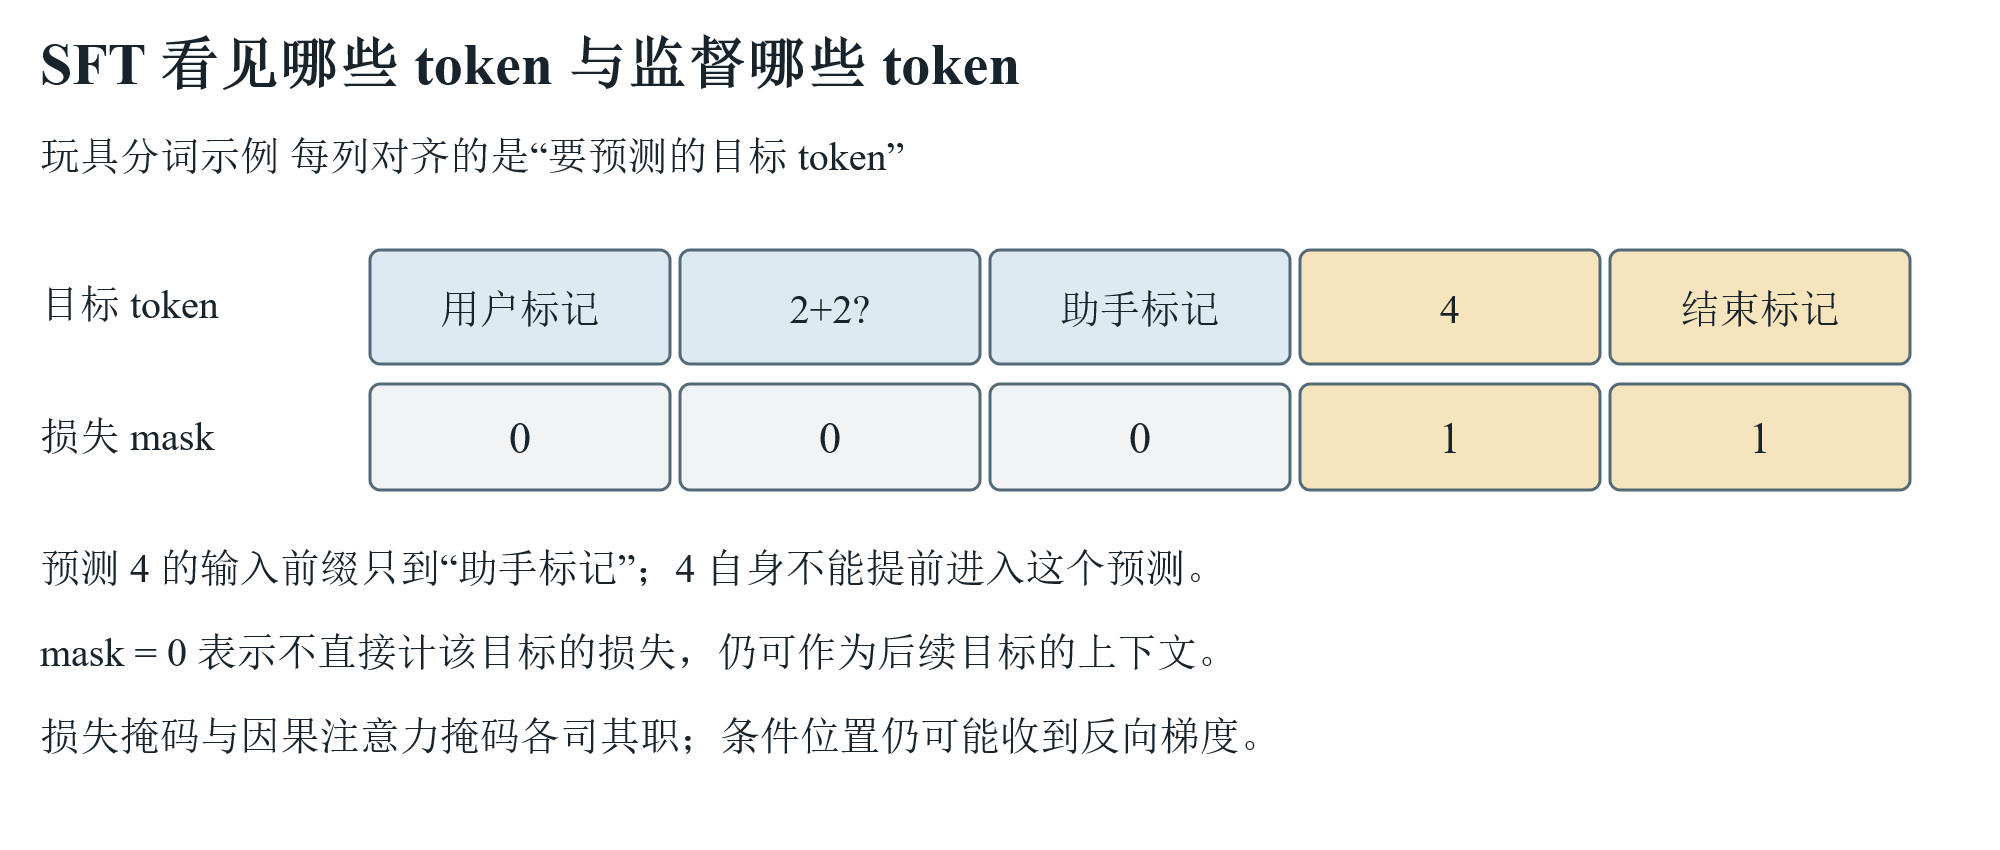
\includegraphics[width=\linewidth]{assets/media/image12.png}
    \caption{一条 SFT 样本的目标与损失位置。用户 token 即使不直接计损失，仍能作为助手回答的条件，其相关参数也可能经后续回答损失收到梯度。真实分词和模板可能拆成更多 token。}
    \label{fig:SFT监督位置}
\end{figure}

从行为克隆（behavior cloning）的视角，SFT 告诉模型``遇到这里，示范者这样走''。示范由外部给定，在本书的宽泛用法中属于异策略（off-policy）数据；它与学生当前生成的路径可能不同。它没有显式要求模型在多个候选中评判哪个更好。可我们也不能说它绝对学不到判断：若数据里包含批改、比较和自我纠错示范，模型同样可以学习这些行为。真正的区别是，普通最大似然并未直接优化独立的偏好比较或环境回报。

训练后，小助开始稳定给出分步答案。我们很高兴，却先在验证集核对：是否只学会了固定套话？是否每题都添加无意义检查？是否在资料不足时照样编造？格式是容易观察的进步，任务能力与可靠性还需要分别检查。

\textbf{实践}~注意，从这里开始就进入模型训练部分，推荐读者能够对每一个训练方法有一定的自主实践，后续大多数章节中不再单独给出实践建议。

\textbf{本节相关资料}
\begin{enumerate}
    \item Ouyang 等，2022，\href{https://arxiv.org/abs/2203.02155}{Training language models to follow instructions with human feedback}。即 InstructGPQ，前面多次参考到。阅读重点：监督示范在整个反馈训练管线中承担什么作用。
    \item Wei 等，2021，\href{https://arxiv.org/abs/2109.01652}{Finetuned Language Models Are Zero-Shot Learners}，FLAN 。阅读重点：任务多样性如何帮助指令泛化。
\end{enumerate}

\section{SFT 数据工程 模板与监督位置}\label{SFT 数据工程 模板与监督位置}

我们准备扩充 SFT 数据。最容易的做法是搜集尽可能多的问答，却发现质量逐渐失控：有的答案只给数字，有的先闲聊，有的把推理写错，有的缺少轮次结束标记。

我们先规定示范质量。方程题要求步骤正确、足够解释且不编造定理；资料题要求引用可找到、依据能支撑回答；信息不足题要求说明缺少什么。我们可以保留不同的表达方式，避免把多样性误当成噪声，但不保留彼此矛盾的任务要求，比如同一个问题我们给两种截然不同回答风格：一个花非常大的努力做深度推理，采样到一个非常长而详细的回答，另一个尽可能节约推理成本，尽量少验证，快速给出答案。模型对于同一个题目学习这两种完全不同风格的回答，就会导致行为冲突，具体可能表现为 grad norm 或者 loss 出现尖峰（spike），并且在训练完以后在推理时出现严重的复读现象。这体现出数据清洗的重要性。

训练前，我们随机抽取已 token 化的样本，检查角色边界、监督位置、最大长度与结束标记。若长样本总在最终答案之前被截断，小助就可能学会漫长推演，却学不到收束推导。

我们也会看分项损失。固定模板词频很高，模型很快学会``下面分步骤说明''这种习惯，总 loss 因此下降，但真正关键的算术 token 改善有限。这不表示格式一定``劫持''了学习，而是平均指标掩盖了不同位置的难度与价值。为了追求严谨，应该把格式正确率、答案正确率、步骤有效率都作为监控指标，防止只优化其中最容易的一项。

计算资源有限时，我们可以使用低秩适配（Low-Rank Adaptation，LoRA）。它冻结大部分基础权重，用低秩增量表达参数更新，减少可训练参数和优化状态。这个方法的思路非常简单但是非常重要，推荐读者自学，主要关注两点：一是如何节约计算开销，二是为什么 LoRA 单训一批小数据不太造成灾难性遗忘\footnote{灾难性遗忘是指这种现象：一个经过后训练的大模型在各方面能力达到均衡，此时用一个专项领域数据继续 SFT，导致其他各方面能力明显下降。这是许多任务里面需要考虑的问题。}。LoRA 解决的是适配成本与参数化方式，主要是大幅节约计算资源，无法修复坏数据，也不保证没有灾难性遗忘。秩（rank）、作用模块、学习率和数据量仍需要验证。全参数微调也并非总优于 LoRA，两者优劣应在清楚的预算和任务下进行\footnote{LoRA 系列方法在学术界受欢迎，因为计算开销大幅下降，可以做很多训练，但是在工业界大多不被支持，一方面是因为工业界有充足的数据资源和计算资源，二是因为对于各家自研模型来说，训练框架越简单越好，功能越少越好，否则难以维护，在这种情况下，LoRA 训练通常不被支持。}。

第一次小规模训练，我们故意让模型在少量干净样本上过拟合。若连这一步都做不到，先查管线；若可以学会，再扩大数据，观察泛化能力。任何系统性工程任务都需要预实验，对模型的上限和下限都有所了解。

\textbf{本节相关资料}
\begin{enumerate}
    \item Zhou 等，2023，\href{https://arxiv.org/abs/2305.11206}{LIMA Less Is More for Alignment}。比较有名的论文。阅读重点：高质量少量示范数据的训练价值可能非常大；但是也不要认为``少量数据总是足够''。
    \item Hu 等，2021，\href{https://arxiv.org/abs/2106.09685}{LoRA Low-Rank Adaptation of Large Language Models}。\textbf{（务必理解LoRA原理）}阅读重点：低秩更新节省了哪些资源，又没有保证哪些能力。即便不看论文原文也建议找资料理解 LoRA 如何高效训练。
\end{enumerate}

\section{续训退化 新任务变好为何旧能力变差}\label{续训退化 新任务变好为何旧能力变差}

小助已经会耐心讲题，我们想加入一门新课程，于是准备一批领域问答继续 SFT。为了节省标注，答案几乎都是一句话：``答案是 5。''\,``定义见第三章。''\,``选择 B。''新课程题的分数上升了，但小助对旧题也开始只给结论，不愿解释。

小助可能仍然有能力解释这些问题，只是在新训练分布下更偏向简短回答；也可能失去了某些步骤能力，这就是``灾难性遗忘''；也可能是对话模板变了（很少出现这种失误）。

更新为什么会波及旧任务？不同任务共享大量参数。新数据的梯度鼓励短答案，可能降低长解释的概率；新领域的词汇、格式、难度与采样比例，也会重新分配训练权重。

训练强度同样关键，通常学习率是 8e-5。相同的新数据，较高学习率、更多轮次的训练，都可能造成更大的参数漂移。反过来，过低学习率（比如 2e-5）也可能学不到新增任务。我们不能只说``把学习率调小''，而要在新任务收益和旧任务保留之间做曲线比较，用实验结果来验证猜想，合适的参数通常需要多组训练后测试结果然后对比观察，经验丰富的工程师通常有较好的参数直觉。

怎样区分``不再主动解释''和``已经不会解释''？我们用同一批旧题，对比续训前后模型在三种条件下的表现。以方程题 $3(a+2)=21$ 为例：第一种只问``求 $a$''；第二种明确要求``请逐步求解，并代回原式检验''；第三种再提供一个正确的起步提示，例如``先把等式两边除以 3，得到 $a+2=7$，请继续求解并检验''。除了最终答案是否正确，还要分别检查步骤和检验过程是否正确。

如果续训后的模型在普通提问下只给答案，但在第二种条件下仍能正确解释和检验，说明相关能力至少仍能被明确指令调动出来，退化可能主要表现为默认回答方式变了。如果第二种条件下做不好，第三种条件下却能完成，说明它在获得提示后仍能接着做，但独立组织完整解答的表现有所下降；不能据此说它毫无退化，也不能说它已经完全不会做。

如果连第三种条件下也频繁失败，而续训前的模型在相同条件下能稳定完成，我们才有更充分的理由怀疑相关任务能力受到了损害。这里比较的是一批题上的正确率，而不是某一道题的一次回答；测试时也要保持对话模板、生成长度限制等条件一致，避免把提示差异或回答被截断误判为遗忘。

\textbf{一个具体案例：知道相关信息，却说不出完整姓名。}MiniMax 报告过这样一种异常：模型能回答``马嘉祺''的相关信息，但在被问到``时代少年团的队长叫什么名字''时，却无法输出姓名中的``嘉祺''。在该模型的词表中，``嘉祺''恰好是一个完整的 token，而且在后训练数据中很少出现。

要理解排查方向，需要区分模型的输入端和输出端。输入嵌入把读到的 token 转成向量，供后续计算使用；输出头（LM head）则根据当前的隐藏状态，为词表中的各个 token 打分，进而得到下一个 token 的概率。MiniMax 对比续训前后的参数后发现，输入嵌入变化很小，但``嘉祺''等低频 token 对应的输出头向量发生了明显变化。团队据此判断，问题主要出在生成端：模型仍能利用输入中的相关信息，却更难在回答中选中这些 token。

团队随后在 SFT 数据中混入覆盖词表的合成数据，让原本很少作为答案出现的 token 也有机会成为训练目标，并报告上述姓名生成及部分词语复制问题得到改善。这个案例与前面的诊断方法相呼应：先确认模型究竟在哪个环节失败，再选择修复手段。

这时我们也重新考虑方法的选择。若希望模型掌握经常变化的课程规则，采用RAG 方法也许比把每条规则写（训练）进权重更合适；若要长期改变模型的语言风格，SFT 更直接。继续训练之前，我们必须明确目标：希望模型新增知识还是改变行为，或者想都实现。

\textbf{本节相关资料}
\begin{enumerate}
    \item Kalajdzievski，2024，\href{https://arxiv.org/abs/2401.05605}{Scaling Laws for Forgetting When Fine-Tuning Large Language Models}。阅读重点：微调收益与原能力保留如何随训练条件变化。
    \item Wu 等，2023，\href{https://arxiv.org/abs/2310.00492}{From Language Modeling to Instruction Following Understanding the Behavior Shift in LLMs after Instruction Tuning}。阅读重点：指令微调前后的行为变化应如何测量。
    \item MiniMax Research，2026，\href{https://www.minimax.cn/blog/sparse-token-forgetting-investigation}{为什么 MiniMax 大模型不认识``马嘉祺''？稀疏 Token 遗忘排查记录}，研究博客。阅读重点：如何从姓名生成失败出发，对比输入嵌入与输出头的变化，再用词表覆盖数据检验修复方向；注意区分案例观察与普遍结论。
\end{enumerate}

\section{遗忘诊断 用对照实验选择修复方法}\label{遗忘诊断 用对照实验选择修复方法}

发现旧任务表现下降以后，我们先不要急着补数据或调学习率。``旧能力变差''只是现象，背后可能是示范风格改变、训练更新过强，也可能是模板或截断问题。不同原因需要不同处理。如果同时换数据、改模板、调学习率，即使下一次结果变好了，也很难知道究竟是哪一步起了作用。

\textbf{先固定起点和评估方法。}我们回到续训前的同一个检查点\footnote{检查点是训练过程中保存的模型状态。}，再分别启动后续实验。不能先训练 A 组，再从 A 组的结果接着训练 B 组，然后把两者当作只有数据不同的对照：B 组已经多经历了一段训练，起点就不一样了。

我们准备互不混用的训练集和评估集。新课程评估集检查新任务是否学会，旧任务评估集检查原有表现是否保留；评估题不能直接作为回放样本加入训练，否则可能只是把考题记住了。旧题还要按前一节的方法，区分普通提问、明确要求解释、提供起步提示这几种条件，并分别记录最终答案正确率、步骤正确性和检验是否有效。对话模板、生成长度上限和采样设置也应固定，这样不同模型的表现才有可比性。

\textbf{用四组实验分别检验不同解释。}沿用新课程问答的例子，我们先做下面几组小规模实验：
\begin{enumerate}
    \item \textbf{A 组：只用新课程数据，作为基线。}数据仍以简短答案为主，使用事先确定的训练设置。它回答的是：按照原方案继续训练，新任务能提高多少，旧任务会下降多少？。
    \item \textbf{B 组：混入旧任务示范。}旧示范覆盖我们希望保留的代表性任务，例如分步解方程、代回检验、资料不足时说明限制。这种把以前任务的数据重新放进训练的做法叫作回放（replay）。它检验的是：新数据中缺少旧任务信号，是否参与了退化？混入比例要预先记录，例如按训练 token 计，旧数据占总量的十分之一。
    \item \textbf{C 组：保持 A 组的数据和训练步数，只降低学习率。}这样主要检查单次参数更新的强度是否过大。如果还想研究训练轮数，就另开一组，只减少轮数而保持学习率不变。
    \item \textbf{D 组：修改新课程示范的回答方式。}保留相同的题目和任务要求，把只有结论的答案改成包含必要步骤和检查的答案，并审核其正确性。它检验的是：新数据是否把``所有问题都简短作答''这种习惯一起教给了模型？但补充讲解也会增加训练 token，所以比较时必须同时记录数据长度和训练预算。
\end{enumerate}

这里的``每次只改一个因素''，指的是先明确每组在检验什么假设，并尽量控制其余条件。数据改动往往会连带改变长度、采样次数和计算量，做不到只写一句``其他条件相同''就忽略它们。把这些变化记录清楚，本身也是实验设计的一部分\footnote{在实际工作里面，因为计算资源、时间等有限，我们很难有充足时间去单变量调整，所以建议在学习时多实验多积累经验。}。

\textbf{说清楚训练预算按什么对齐。}以 B 组为例，如果 A 组训练了 100 万个新任务 token，B 组也训练这 100 万个新任务 token，再额外加入 10 万个旧任务 token，那么 B 组使用了更多计算。即使它表现更好，也不能直接说明在相同预算下混合数据一定更优。另一种比较是把两组都限制为 100 万个训练 token，B 组分配 90 万个给新任务、10 万个给旧任务。这更接近固定预算下的数据分配问题，但 B 组见到的新任务数据又少了。

这两种比较都有意义。前者问的是``为了保留旧能力，额外付出一些训练成本是否值得''；后者问的是``总预算不变时，怎样分配新旧数据''。我们应先选定要回答的问题，再解释结果。

\textbf{把实验结果当作线索，再回到具体样本。}假设这次实验出现以下现象：
\begin{itemize}
    \item A 组新题正确率上升，但旧题的步骤正确性下降，说明原训练方案确实存在需要处理的取舍；它本身还不能告诉我们原因。
    \item B 组比 A 组保留了更多旧任务表现，支持``补充旧任务训练信号可能有帮助''这一判断。若比较预算不同，还要考虑额外计算或新任务训练量减少的影响。
    \item C 组旧任务退化较少，但新任务收益也变小，说明减小更新可能缓和退化，同时也可能让新任务学得不够。我们应比较不同训练阶段的结果，寻找满足需求的检查点，而不是只看最后一次保存的模型。
    \item D 组在新旧题上都更愿意解释，而且解释正确率提高，支持继续检查示范风格的影响。若只是字数变多、步骤仍然错误，就不能算作能力恢复。
\end{itemize}

结果接近时，也不要过早排序。我们可以换一批留出题复查，或者在资源允许时更换随机种子重复训练，观察结论是否稳定。小评估集上的少数题变化、随机采样的偶然成功，都可能让某一组看起来更好。

接下来逐条检查失败样本。若答案正确、只是解释变短，而且明确要求后能恢复，就优先检查示范风格；若新课程和旧课程使用不同规则，模型却混用规则，就检查题目是否明确标出了课程或适用条件；若回答总在中途结束，就检查最大生成长度、训练样本截断，以及结束标记是否被放错。尤其是最后一种情况，先修正数据或推理管线，比继续增加训练量更直接。

\textbf{让修复方法对应已经观察到的问题。}回放的作用，是在学习新任务时继续提供以前其他学过的任务数据的监督信号。但旧数据不是随便抽一些就够了：如果只回放简单算术，不能指望它同时保住长文讲解和资料引用。我们需要按实际关心的能力选择代表性样本，再在没有参与训练的旧题上验证效果。回放比例过大也会挤占新任务的训练预算，因此仍要比较新旧任务的收益。

另一种方法是保留一个冻结的参考模型，例如续训前的模型。对同一段旧任务上下文，让当前模型和参考模型分别预测下一个 token；除了学习新示范，还加入一项损失，惩罚两者预测分布相差太大（即尽可能稳健更新）。这类约束常用 KL 散度衡量，直觉上就是：在希望保留的旧场景中，先别偏离原模型太远。这里约束的是预测行为，不是要求所有参数保持原值。它需要额外的参考模型计算，而且约束过强会妨碍新任务学习；参考模型原有的错误也可能被保留下来。下一章会进一步介绍 KL 约束。

如果旧任务示范不足，也可以请一个经过验证的教师模型生成解答，再审核、筛选成训练数据。这样给学生模型提供的是可模仿的完整示范；前面比较预测分布的方法则提供更细的概率信号，两者不能笼统地用``老师给反馈''一笔带过。无论采用哪一种，教师也可能答错，训练数据覆盖不到的任务也仍可能退化，最终都要靠独立评估检查。

最后，新旧目标有时确实冲突。例如同一类问题，在完全相同的输入条件下，旧任务要求详细讲解，新任务却要求只输出一个选项。如果不给出区分条件，模型无法同时把这两种回答都当作唯一要求。此时应先在指令中明确任务模式，或者重新确定产品需求；单靠增加回放或减小学习率，不能消除要求本身的矛盾。

这一轮工作的顺序是：先定义下降的是哪项表现，再提出可以检验的原因，设计可比较的小实验，结合指标和失败样本选择修复方法，最后扩大数据与训练预算。只有确认改动在留出题上有效，我们才有理由把它用于下一轮训练。

在真实的实验、工作场景中，训练可能会出现各种各样的问题，例如 Loss 曲线或者 Grad norm 曲线出现严重的 spike，或者 Loss 曲线起步时数值偏高，训练完之后模型的复读率提高等，都是在学术研究时容易忽略的问题，读者可以自己查阅资料思考这种情况的原因和解决方案。

\textbf{实践}~参考一些开源学习项目，在服务器上用 LoRA 方法 SFT 后训练一个 Qwen 小模型，观察训练前后模型的某些能力是否像预期一样变化。

\textbf{本节相关资料}
\begin{enumerate}
    \item Kalajdzievski，2024，\href{https://arxiv.org/abs/2401.05605}{Scaling Laws for Forgetting When Fine-Tuning Large Language Models}。阅读重点：研究如何定义和测量遗忘，比较哪些训练条件；注意 LoRA 也不保证保留全部旧能力，论文中的观察仍需结合具体实验范围理解。
    \item Hinton 等，2015，\href{https://arxiv.org/abs/1503.02531}{Distilling the Knowledge in a Neural Network}。阅读重点：教师模型的预测分布为什么能成为学生模型的训练信号。这是理解知识蒸馏的基础资料，并非本节所有遗忘修复方法的直接实验依据。
\end{enumerate}